\documentclass[12pt, onecolumn]{IEEEtran}
\usepackage{graphicx, caption}
\begin{document}

%don't want date printed
%make title bold and 14 pt font (Latex default is non-bold, 16 pt)
\title{\Large \bf Large Scale Data Mining\\ Homework 3\\Collaborative Filtering}
\author{
{\rm Anurag Pande - 604749647}\\
{\rm Brendon Faleiro - 704759004}\\
{\rm Sachin Krishna Bhat - 304759727}
}

\maketitle
\section{Introduction}
Collaborative Filtering refers to the method of predicting a user's opinion based on an entity using other users' opinions. These methods are based on the notion that there exist other users with behavior similar to our target user and by finding and observing these users we can predict the target user's behaviour.\\
To understand Collaborative Filtering we were provided with the MovieLens dataset consisting of 100k ratings. These ratings were composed of 943 users and 1682 movies.\\
\section*{Question 1: Matrix Factorization}
To factorize the data, we first analyzed the information avaiable in the dataset. We created a matrix R that contained the ratings. The rows of matrix R corresponded to the user\_id and columns corresponded to the movie\_id. As mentioned above, the dataset contained 943 users and 1682 movies. Thus R consisted of 943 rows and 1682 columns.\\
\\
Each entry into R signified the rating given to that movie. So an entry R[i][j] would signify the rating given by user i to movie j. If R[i][j] was marked NaN, it would mean that user i had not yet rated movie j. Since most users had only rated a few movies, the data consisted of a large number of NaNs.\\
\\
We also built a weight matrix W of same dimensions as R, that consisted of weigts based on whether the user had rated that movie. So if user i had rated movie j, that W[i][j] would be set as 1, else it would be marked as an NaN.  \\
We then had to factorize matrix R into matrices U and V such that the suared error between R and the product of U and V was minimized. To achieve this wnmfrule function from the Matrix Factorization Toolbox\cite{wnmfrule} was used. The R matrix and the dimension k was passed as parameters to the function. The function calculated the least squared error as:\\
\begin{equation}
\centering
min \sum\limits_{i=1}^m \sum\limits_{j=1}^n  w_{ij}(r_{ij} - (UV)_{ij})^2
\end{equation}

The wnmfrule function factorized R into matrix U and V and also returned the residual squared error. This factorization process was repeated for 3 different values of k: [10,50,100].\\

\begin{table}[h!]
\centering
\resizebox{0.6\textwidth}{!}{
\begin{tabular}{||c|c|c|c||}
\hline
Dimension k & Residual Error & Squared Error & Iterations \\
\hline\hline
10 & 246.210 & 60619.425 & 100\\
50 & 173.587 & 30132.499 & 100\\
100 & 139.200 & 17213.365 &100\\
\hline
\end{tabular}
}
\end{table}

As can be seen, as the value of k was increased, the error decreased. The best least squared error was observed at k=100.

\section*{Question 2: Cross Validation of the Recommendation System}
The recommendation system designed was then tested using the 10-fold Cross-Validation system that splits the data into 10 parts and uses 9 parts as training data and the 10th part as testing data.\\
\\
We first created a random ordering of indices ranging from 1 to 100k using the \emph{crossvalind} function. This random ordering was used to perform the 10-fold Cross-Validation.\\
\\
We again calculate the factors of R for different values of k as in part 1. This was then compared against the testing data to calculate the absolute error for each fold.\\
\\
The average, maximum and minimum error for each of the 10 folds is shown below.\\
\begin{table}[h!]
\centering
\resizebox{0.6\textwidth}{!}{
\begin{tabular}{||c|c|c|c||}
\hline
Dimension k & Average Error & Maximum Error & Minimum Error \\
\hline\hline
10 & 0.8657 & 0.9106 & 0.7913\\
50 & 0.8717 & 0.9124 & 0.7935\\
100 & 0.8722 & 0.9151 & 0.7990\\
\hline
\end{tabular}
}
\end{table}

As can be seen, the average and maximum errors declined sharply. However, the minimum error remained in the same range with a slight increase in value as the value of k was increased.
\vspace{0.5cm}
\section*{Question 3: Comparing the predicted and observed entries}
Based on the tests from part 2, we try to predict how many people would like the movie. We then calculate the precision and recall values. We also plot the ROC curve for different values of the threshold for the designed recommendation system.\\
\\
We consider 50 threshold values between 0.1 and 5 for the predicted values of the ratings. For actual ratings we use a threshold of 3, and calculate the related precision and recall values. \\
\\
The following graphs show the variation in precision and recall values for different values of k.\\
\\
\textbf{For k=10}
%PUT ALL THE GRAPHS HERE
\begin{figure}[h!]
\centering
\begin{minipage}{.5\textwidth}
\centering
\captionsetup{justification=centering}
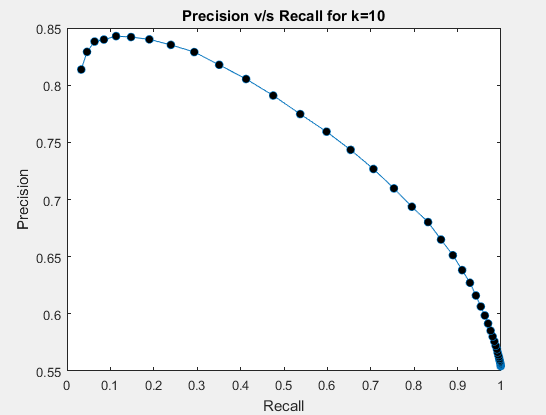
\includegraphics[width=0.9\linewidth]{Graphs/3-1}
\caption{Precision vs Recall}
\end{minipage}%
\begin{minipage}{.5\textwidth}
\centering
\captionsetup{justification=centering}
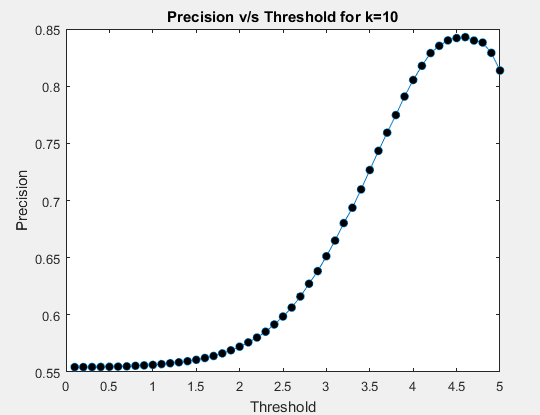
\includegraphics[width=0.9\linewidth]{Graphs/3-4}
\caption{Precision vs Threshold}
\end{minipage}
\end{figure}

\begin{figure}[h!]
\centering
\captionsetup{justification=centering}
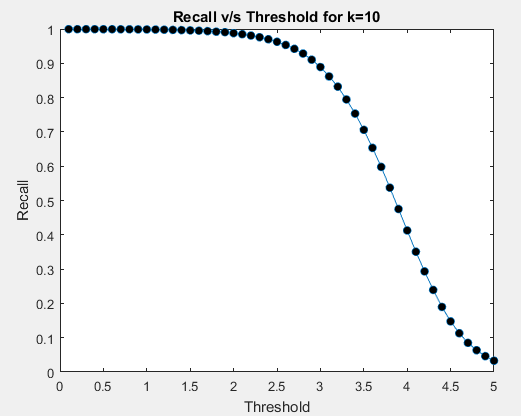
\includegraphics[scale=0.59]{Graphs/3-7}
\caption{Recall vs Threshold}
\end{figure}
\newpage
\textbf{For k=50}
\begin{figure}[h!]
\centering
\begin{minipage}{.5\textwidth}
\centering
\captionsetup{justification=centering}
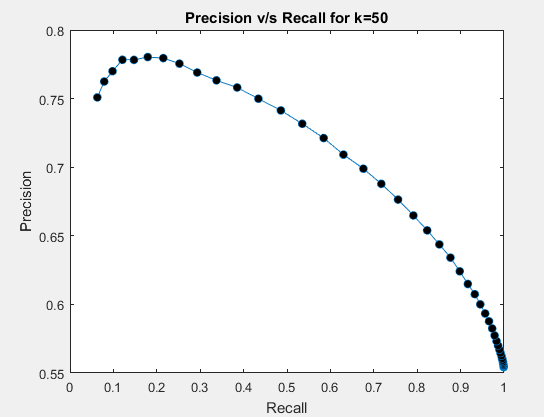
\includegraphics[width=0.9\linewidth]{Graphs/3-2}
\caption{Precision vs Recall}
\end{minipage}%
\begin{minipage}{.5\textwidth}
\centering
\captionsetup{justification=centering}
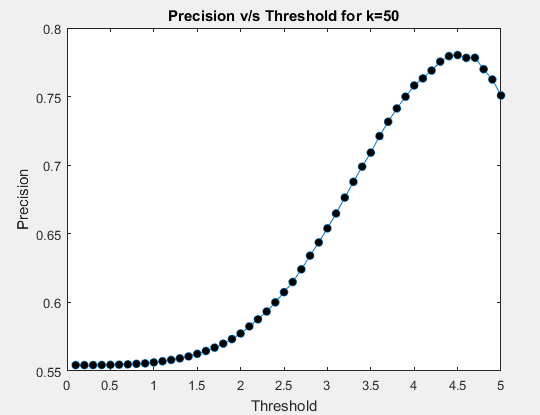
\includegraphics[width=0.9\linewidth]{Graphs/3-5}
\caption{Precision vs Threshold}
\end{minipage}
\end{figure}
\begin{figure}[h!]
\centering
\captionsetup{justification=centering}
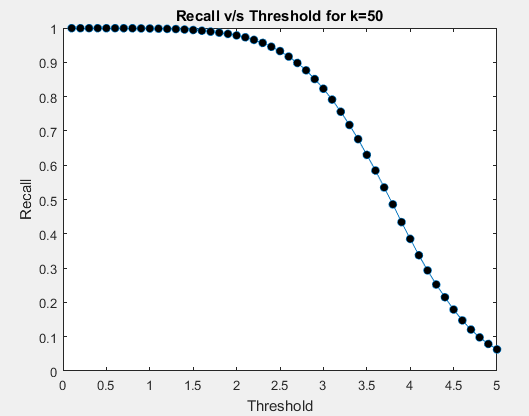
\includegraphics[scale=0.59]{Graphs/3-8}
\caption{Recall vs Threshold}
\end{figure}
\newpage
\textbf{For k=100}
\begin{figure}[h!]
\centering
\begin{minipage}{.5\textwidth}
\centering
\captionsetup{justification=centering}
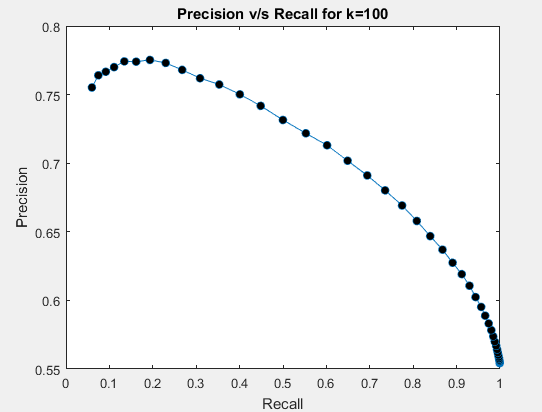
\includegraphics[width=0.9\linewidth]{Graphs/3-3}
\caption{Precision vs Recall}
\end{minipage}%
\begin{minipage}{.5\textwidth}
\centering
\captionsetup{justification=centering}
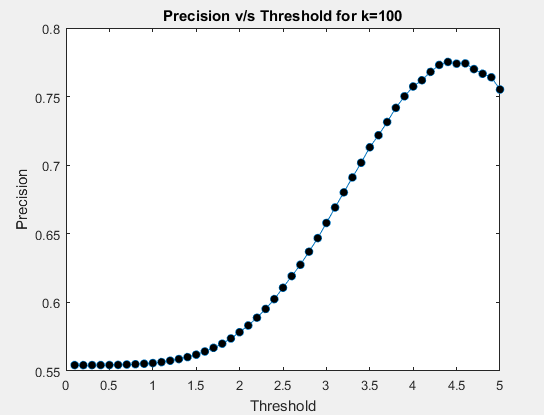
\includegraphics[width=0.9\linewidth]{Graphs/3-6}
\caption{Precision vs Threshold}
\end{minipage}
\end{figure}
\begin{figure}[h]
\centering
\captionsetup{justification=centering}
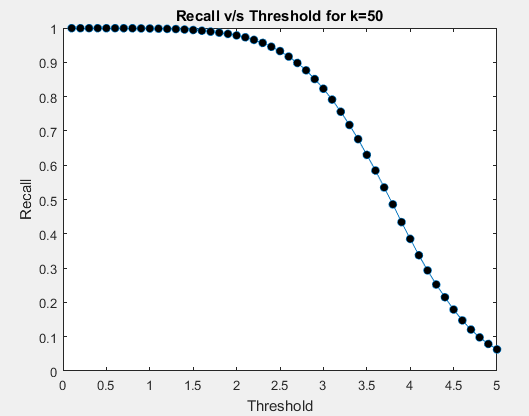
\includegraphics[scale=0.59]{Graphs/3-9}
\caption{Recall vs Threshold}
\end{figure}
%
%
\subsection*{Observations:}
\begin{itemize}
\item Precision decreases as recall increases. As k is increased, the precision vs recall graph becomes steeper.
\item Precision improves with an increase in threshold values. As k is increased, the curve for precision vs threshold becomes steeper.
\item Recall deteriorates as threshold is increased. The curve for recall vs threshold shows that the curve becomes steeper as k is increased.
\end{itemize}
\newpage
\section*{Question 4: Factorizing data with Regularization}
	Now, we change the weight matrix and use rating values as weights, rather than 1. Also the value of the R matrix is set to 1 for known entries and NaN for unknown entries. So, we reverse the roles of R and W in the factorization step. For this new weighted matrix, we calculate the minimum squared error and we find it to be lower than the values from part 1. In order to avoid singular solutions, we modify the cost function by adding the regularization term $\lambda$ . 
	\begin{equation}
	\centering
	min \sum\limits_{i=1}^m \sum\limits_{j=1}^n  w_{ij}(r_{ij} - (UV)_{ij})^2 + \lambda ( \sum\limits_{i=1}^m \sum\limits_{j=1}^k u_{ij}^2 + \sum\limits_{i=1}^k \sum\limits_{j=1}^n v_{ij}^2)
	\end{equation}
	
We then add a regularization parameter as defined in the spec sheet. We chose $\lambda$ to be in the range of values \textbf{\{0.01, 0.1, 1\}}.  This function calculates the values of U and V as:
\begin{equation}
U = U.* (((W.* R) * V')./(\lambda * U + (W .* (U * V)) * V'))
\end{equation}
\begin{equation}
V = V.* ((U' * (W .* R))./(\lambda * V + U' * ( W.* (U * V))))
\end{equation}

We calculate the precision and recall for these lambda values with respect to the latent features. The ROC plots are given below.

\begin{figure}[h]
\centering
\captionsetup{justification=centering}
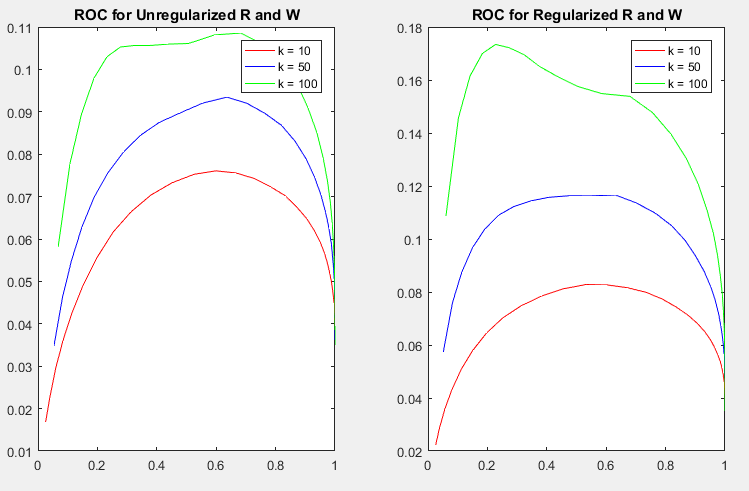
\includegraphics[scale=0.9]{Graphs/ROC1}
\caption{ROC for Regularized and Unregularized R and W}
\end{figure}

\begin{figure}[h]
\centering
\captionsetup{justification=centering}
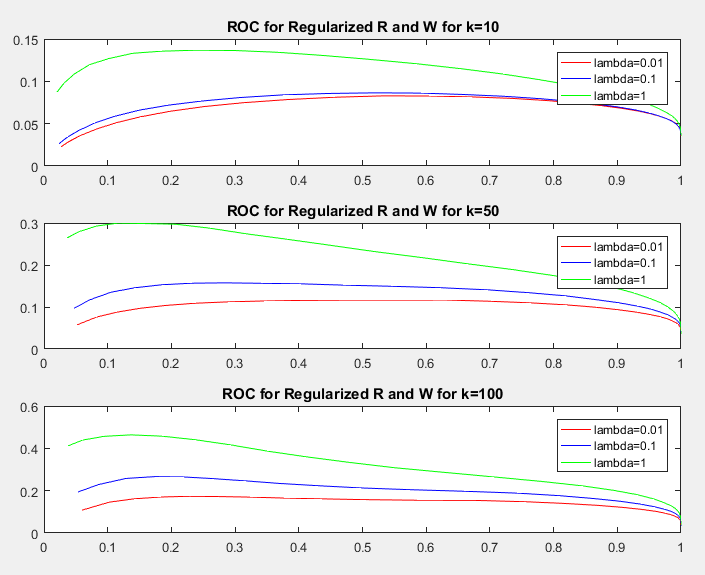
\includegraphics[scale=0.65]{Graphs/ROCregularized}
\caption{ROC for regularized R and W for different Lambda values}
\end{figure}

\begin{figure}[h!]
\centering
\captionsetup{justification=centering}
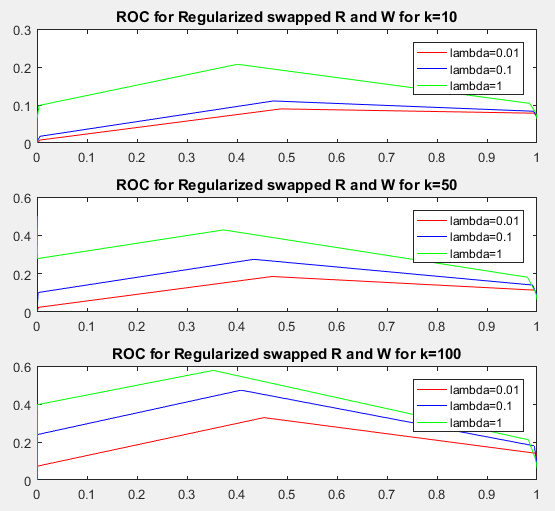
\includegraphics[scale=0.82]{Graphs/swapped}
\caption{ROC for regularized swapped R and W for different Lambda values}
\end{figure}

\newpage
\section*{Question 5}
The main aim is to convert R to a 0-1 matrix where the entries are 1 for the available data points and 0 for the missing data points, and find the top L movies recommended to each user. In this predicted matrix R we replace entries which are not present with -1 as a placeholder to ensure independence of the calculations. Then, the ratings for every user are sorted in descending order to get the top L movies for every user.
\\\\
Then, we execute for every fold and find the precision, ignoring the movies whose ratings are not present in the R matrix (ignoring the placeholder -1 values).
\begin{center}
	Average precision for L = 5 is \textbf{0.5531}
\end{center}

The next thing is to find our algorithm's \textbf{hit rate (equivalent to true positive rate)}. We define hit rate as: 
\begin{equation}
	Hit\ rate = \frac{Suggested\ movies\ liked\ by\ user}{True\ positive + false\ negative }
\end{equation}
We calulate number of movies in L for each user that have a value greater than the threshold. This gives us the hit rate. The false alarm rate is defined as:
\begin{equation}
	False\ alarm\ rate = \frac{Suggested\ movies\ not\ liked\ by\ user}{false\ positive + true\ negative}
\end{equation}
where,\\
true positive = no. of times both actual and predicted ratings are above the threshold\\
true negative = no. of times both actual and predicted ratings are below the threshold\\
false positive = no. of times the actual rating is above the threshold while the predicted rating is not\\
false negative = no. of times the actual rating is below the threshold while the predicted rating is not\\
\\The \textbf{false alarm rate (equivalent to false positive rate)} is comprised of all ratings that are recommended to the user but fall below the threshold.
\\\\	The values of Hit Rate and False Alarm Rate changed as the values of L were varied. We reuse the same R predicted matrix as refactorization is unnecessary.
\begin{figure}[h!]
\centering
\captionsetup{justification=centering}
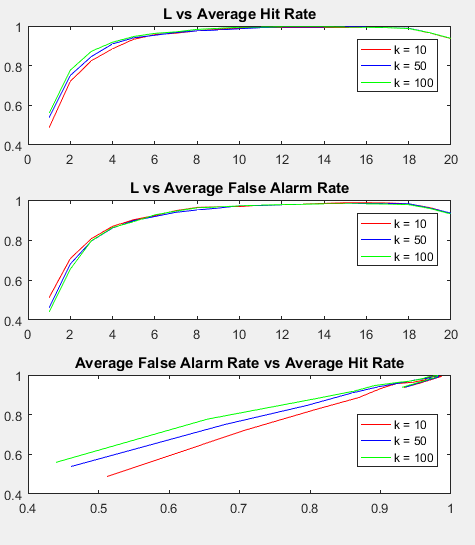
\includegraphics[scale=0.85]{Graphs/5}
\end{figure}

\newpage
\subsection*{Observations}
\begin{itemize}
\item As seen in the figure, as the value of L increases, the Hit Rate tends to approach 1, ie. an optimum solution. As L increases, the scope of the movies that are to be suggested to the user increases. If the value of L exceeds the actual number of movies liked by the user, it reaches a Hit Rate of 1 for that condition.
\item False alarm rate also tends to reach 1. 
\end{itemize}

\begin{thebibliography}{1}

\bibitem{wnmfrule}The Non-Negative Matrix Factorization Toolbox in MATLAB \texttt{ https://sites.google.com/site/nmftool/}

\end{thebibliography}

\end{document}






